\documentclass[twocolumn]{jarticle}
\usepackage[dvipdfmx]{graphicx}
\usepackage{appi2013_2}

%%packages related to equations and math letters
\usepackage{amsmath,amssymb,amsfonts}
\usepackage{amsthm} %定理環境.
%\usepackage{theorem} %定理環境.amsthmを使う場合はコメントアウト.
\usepackage{siunitx} %単位,数値に必要.
\usepackage{latexsym}
\usepackage{empheq} %連立方程式に用いる
%\usepackage{array} %連立方程式に用いる.empheq環境でよい.
%%

%packages related to fonts
\usepackage{bm}
\usepackage{bbm}
\usepackage{otf}
\usepackage[dvipdfmx]{color}
\usepackage[version=3]{mhchem} %化学式を出力するときに用いる.
%\usepackage{newtxtext,newtxmath} %Times フォント関係のパッケージ.
\usepackage{times} % TimesとHelveticaを使う。数式はComputer Modern
%%

%%packages related to structure of the text
\usepackage{ascmac} %make frames
\usepackage{enumerate} %make lists
%\usepackage{enumitem} %customize package of enumerate
%%
%%packages related to quote
%\usepackage{cite}
\usepackage{url}
\usepackage[superscript]{cite}  %参考文献番号を上付にしないなら要らない
\renewcommand\citeform[1]{[#1]} %cite.styを使わないときにはこれもコメントにすること
%%

%%packages related to algorithm and source code
\usepackage{algorithm}
\usepackage{algorithmic}
%\usepackage{listings}
%%

%%packages related to figures and tables
\usepackage{wrapfig}
\usepackage{subcaption}
\usepackage{here}
%\usepackage{multirow}
%\usepackage{slashbox}
%\usepackage{longtable}
%\usepackage{float} %here環境と同じ.使う必要はない.
%%
%%package related to comment
\usepackage{comment} %\begin{comment} ~ \end{comment}でコメントアウトできる.
%%
%%package related to pdf
%\usepackage{pdfpages}

\usepackage{mathtools}
\usepackage[labelformat=parens, justification=raggedright]{subcaption}
% \newcommand{\rfig}[1]{Fig.~\ref{#1}}
% \newcommand{\req}[1]{式\eqref{#1}}
%%command to erase trivial cautions  
% \DeclareFontShape{JY1}{hmc}{b}{n}{<->ssub*hmc/bx/n}{} % Font shape `JY1/hmc/b/n' undefined (Font) using `JY1/hmc/bx/n' instead.のエラーメッセージを消すコマンド.
% \DeclareFontShape{JT1}{hmc}{b}{n}{<->ssub*hmc/m/n}{} %LaTeX Font: Font shape `JT1/hmc/b/n' undefined (Font)	using `JT1/hmc/m/n' instead.のエラーメッセージを消すコマンド.
%%


\jtitle{\fontsize{13pt}{0pt}RDSSAを用いた相互に通信する分子通信系シミュレーション法構築}
\etitle{Construction of Simulation Method for Mutual Molecular Communication System \\ using RDSSA}
\lab{堀}
\no{82411805}
\name{川口竜輝}
\begin{document}
\maketitle

\section{研究背景・目的}
細胞は別の細胞から放出された伝達物質であるシグナル分子が到達すると分子を吸収し,細胞内部で化学反応が発生する.
分子通信系はこの機構を相互に行い,分子数の勾配を情報として伝達する.
分子通信系では,系内部の分子が少数であるため,確率的に反応や分子の到達が発生し,
系内部の細胞濃度が細胞内の状態に影響を与えることが知られている\cite{Yamagishi}.
しかし,この現象をシミュレーションする手法は系の空間全体をシミュレーションするため計算時間が長いという課題があった.
そこで,シグナル分子の到達細胞内部の分子数変化を高速に計算するシミュレーション法\cite{hara}が構築されたが,
送信細胞と受信細胞が区別されているため,双方向の通信ができないという問題があった.
そこで,本研究ではシグナル分子が到達する確率分布が分子の放出時刻
だけ時間変化する点に着目し,計算した確率分布を
相互に通信する分子通信系のシミュレーション法を提案する.

\section{相互通信可能な分子通信系}
1次元の分子通信系において,時刻$t=t_0$に放出された分子が時刻$t$,位置$[\xi,\xi+d\xi)$に存在する確率を
$p(\xi,t|t_0)$とするとき,$p(\xi,t|t_0)$は拡散方程式に従い,分子が位置$\xi =\xi_1$に到達する確率$F(t)$は
\begin{equation}
    F(t) = 1- \int_{-\infty}^{\xi_1} p(\xi,t|t_0)d\xi
\end{equation}
である.ここで,時刻$t=0$に放出された分子が時刻$t$,位置$[\xi,\xi+d\xi)$に存在する確率を
$p_0(\xi,t)$とするとき,$p(\xi,t-t_0|t_0)=$$p_0(\xi,t)$
が成立するため,分子の到達確率分布は放出時刻だけ時間移動する.
この性質を利用し,受信細胞で生成されたシグナル分子の放出時刻を用いて到達確率分布を計算することで相互通信する分子通信系のシミュレーションを構築する.

\section{数値例による検証}
Fig. \ref{fig:image}にあるように,細胞が2つ存在する1次元の分子通信系を考える.ただし,系の拡散係数$\mu=$$\SI{3.0e-4}{\milli\meter\squared\per\minute}$,細胞間距離を$L$とする.
ここで細胞1内部には分子$\mathrm{A}$,$\mathrm{B}$,$\mathrm{X}$,$\mathrm{B:B}$が存在し,次の細胞内部の反応によってシグナル分子$\mathrm{Y}$を放出する.
\begin{equation}
    \emptyset \xrightarrow{k_1} \mathrm{A},\mathrm{X}+\mathrm{A} \xrightarrow{k_2} \mathrm{B}, \mathrm{B} \xrightarrow{k_3} \emptyset, \mathrm{B}+\mathrm{B}\xrightarrow{k_4} \mathrm{B:B} +\mathrm{Y}
\end{equation}
細胞2内部には分子$\mathrm{Y}$が存在し,次の反応によってシグナル分子$\mathrm{X}$を放出する.
\begin{equation}
    \mathrm{Y} \xrightarrow{k_5} \mathrm{X}
\end{equation}
この時,時刻$t=0$において細胞$1$から分子$\mathrm{Y}$が$10^2$個放出されたとき,
細胞$1$,細胞$2$における分子の時間発展を$10^4$回シミュレーションした結果をFig. \ref{fig:simulation} (a)に示す.
ただし,$k_1 = \SI{0.8}{\per\minute}$,$k_2 = \log(2)/20\ \si{\per\minute}$,$k_3=k_4=k_5=\SI{0.02}{\per\minute}$,$L=\SI{0.1}{\micro\meter}$とした.
Fig. \ref{fig:simulation} (a)より,分子$\mathrm{X}$が遅れて増加していることが確認でき,定性的な結果と一致する.
また,$L=\SI{0.1}{\um},$ $\SI{0.2}{\um},$ $\SI{0.3}{\um},$ $\SI{0.4}{\um},$ $\SI{0.5}{\um}$に対する分子$\mathrm{B}$の時間発展をそれぞれ$10^4$回計算した結果をFig. \ref{fig:simulation} (b)に示す.
Fig. \ref{fig:simulation}より,細胞間距離が短いほど分子$\mathrm{B}$の過渡応答が急峻であり,距離依存性を持つことが確認できる.

\begin{figure}[t]
    \centering
    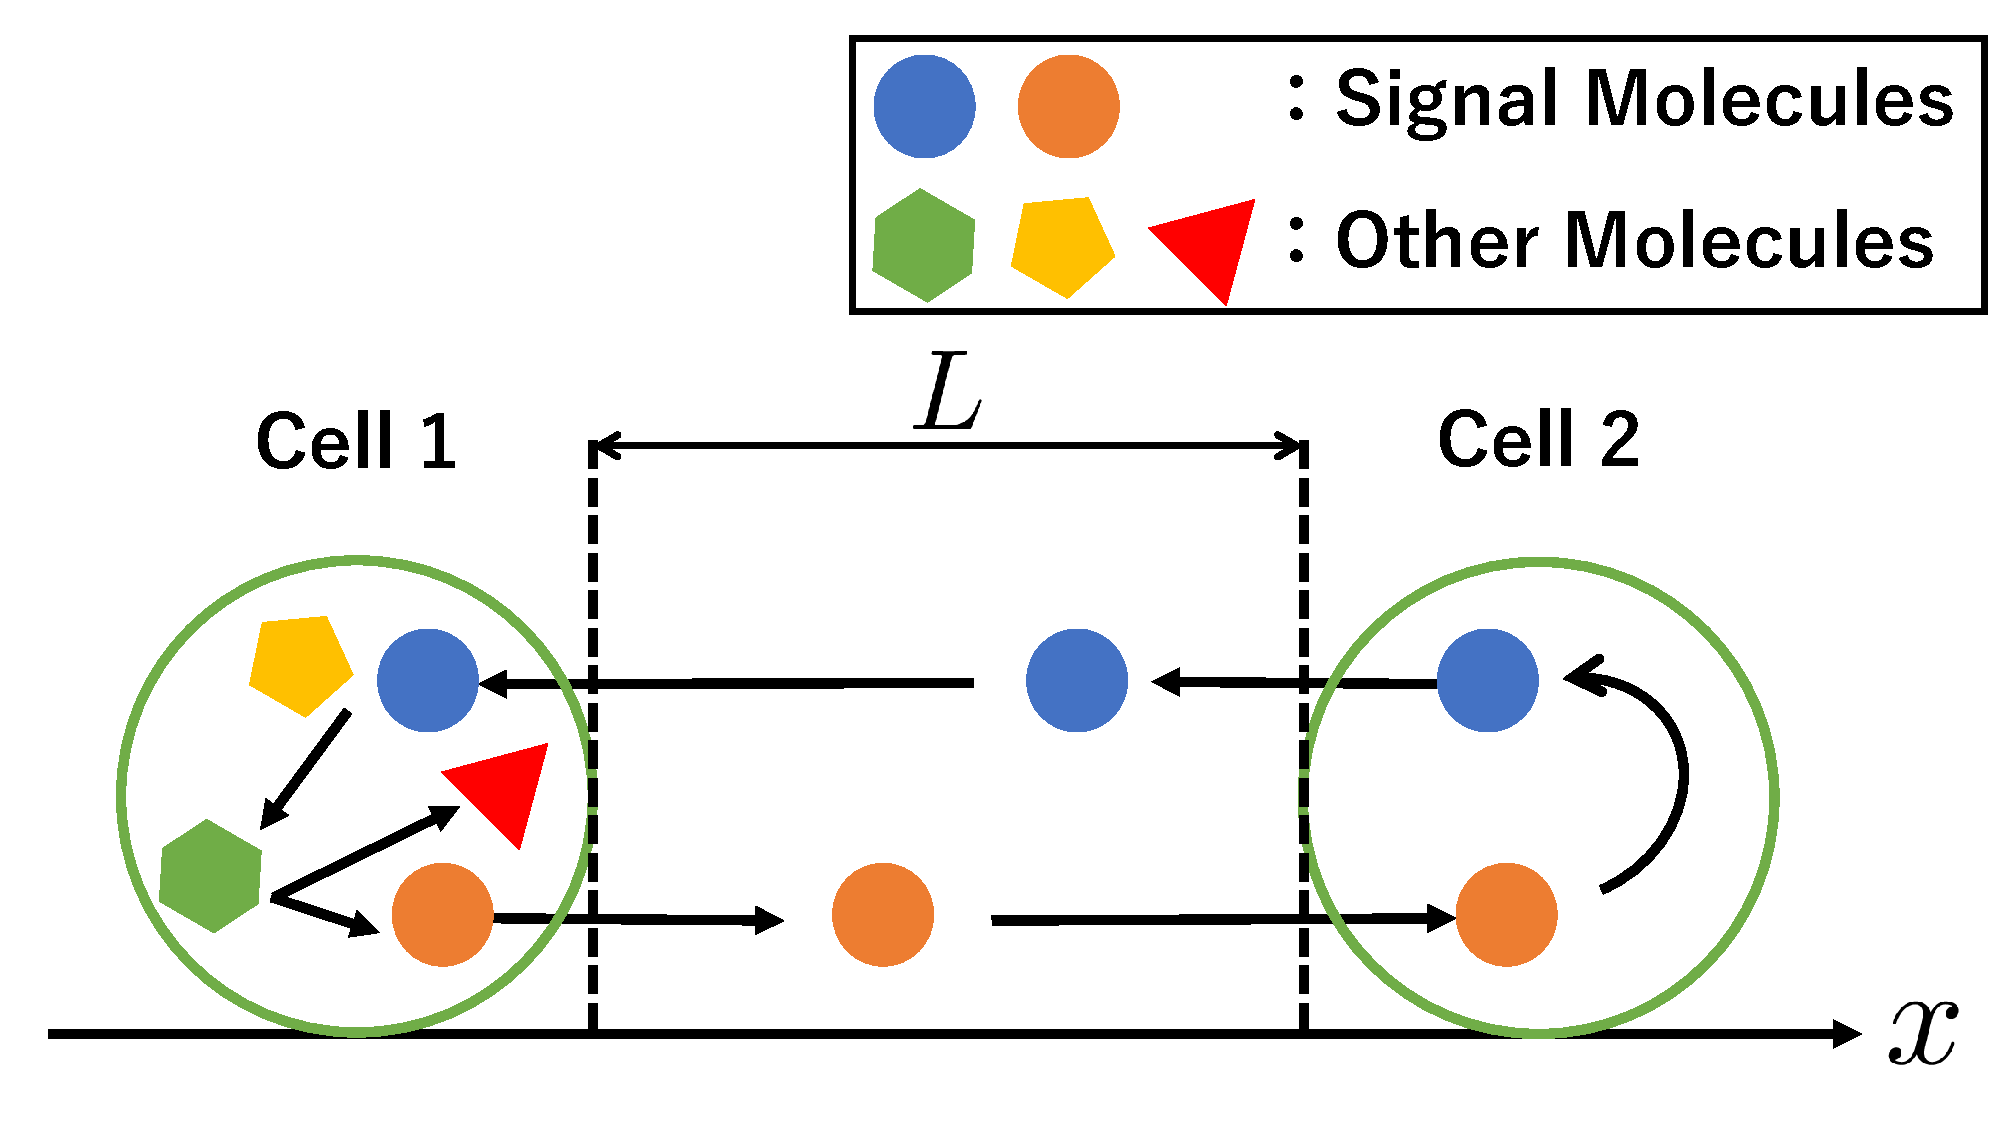
\includegraphics[width=0.8\columnwidth] {figures/Images.pdf}
    \caption{Image of Molecular Communication System}
    \label{fig:image}
\end{figure}
\begin{figure}[t]
    \centering
    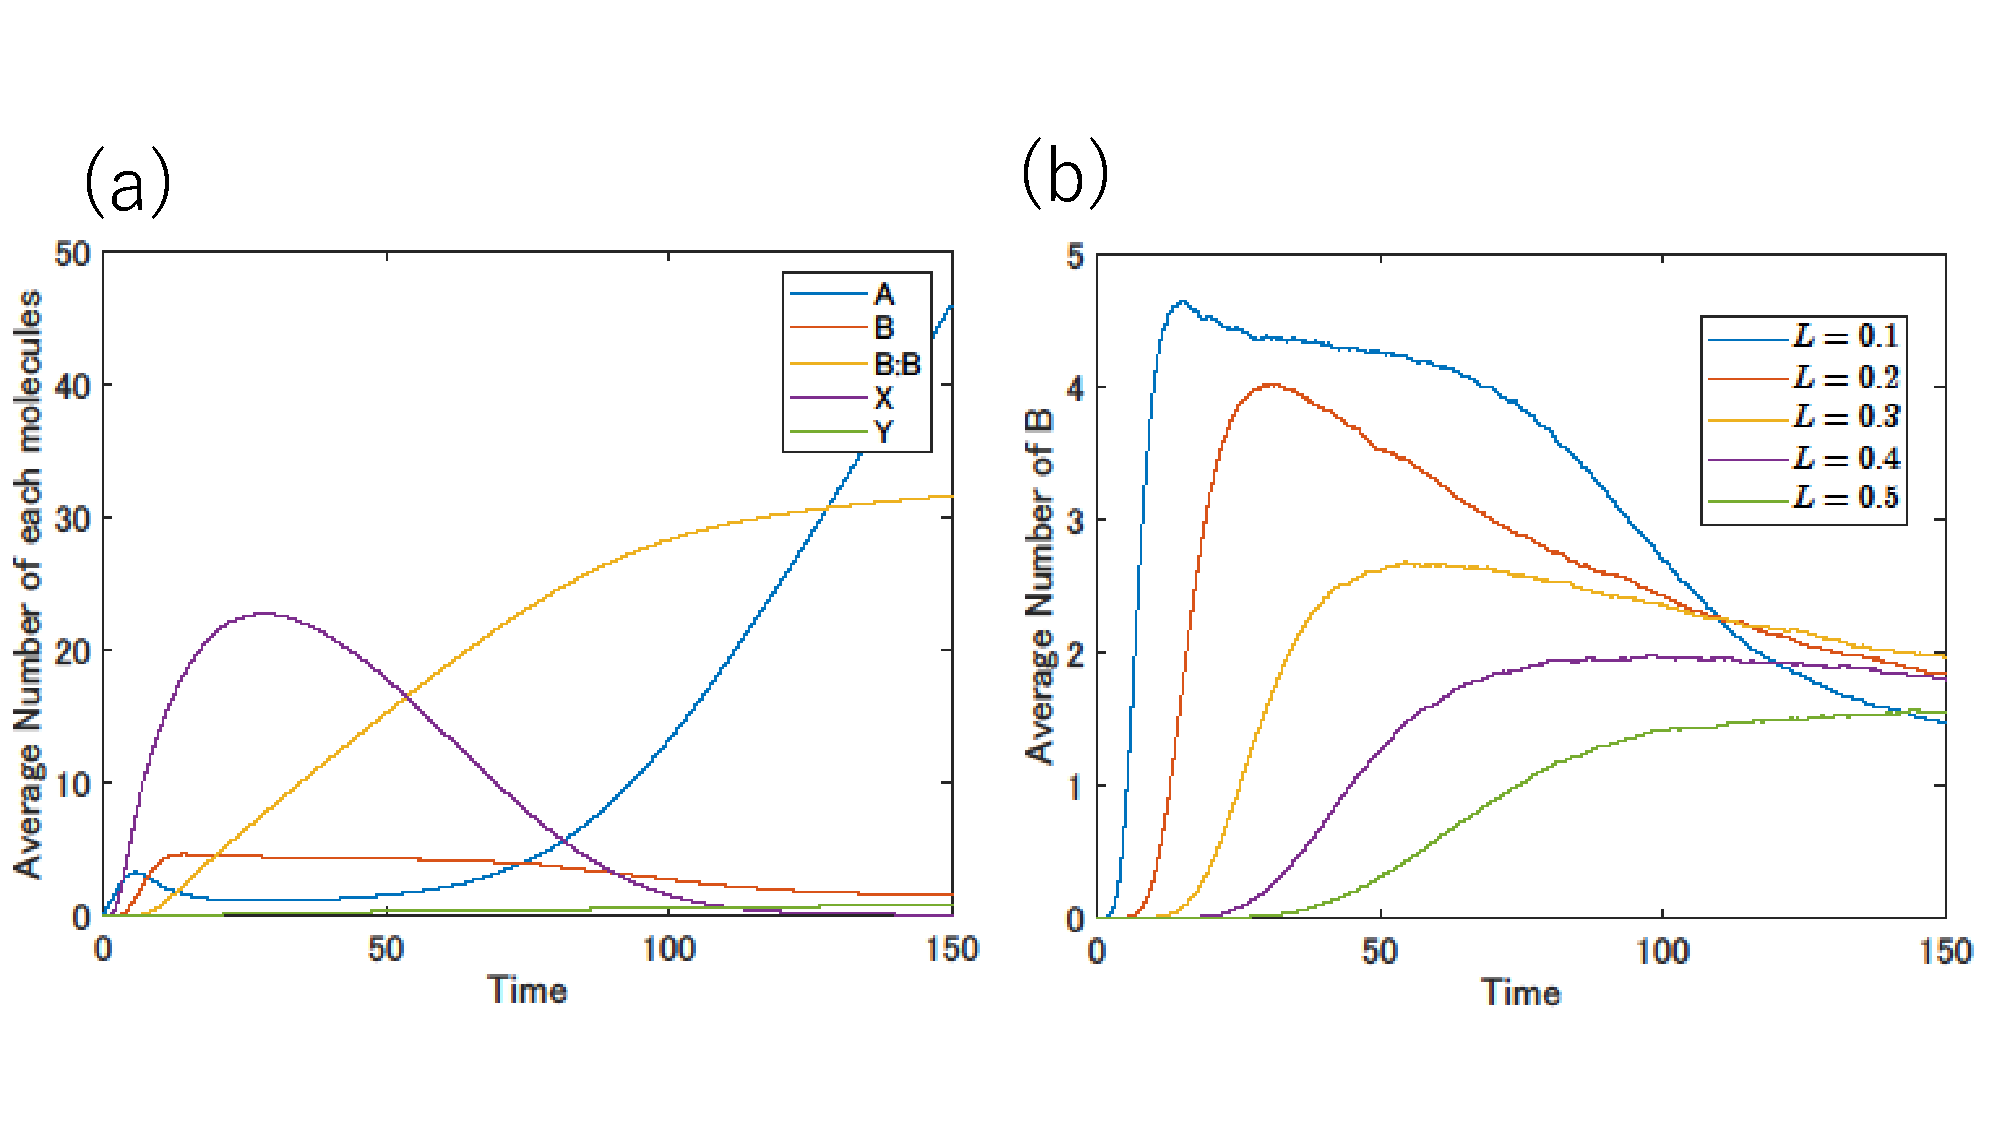
\includegraphics[width=\columnwidth]{figures/simulation_a_and_b.pdf}
    \caption{(a) Time evolution of the average number of each molecules  (b) Comparison of the time evolution of the average number of B among each $L$}
    \label{fig:simulation}
\end{figure}

\section{結論と今後の展望}
本稿では,シグナル分子が到達する確率分布が分子の放出時刻だけシフトすることを利用して
相互通信可能な分子通信系のシミュレーション法を構築した.
今後の展望としては,現在の手法を利用し,2次元の相互通信する分子通信系に対してシミュレーションを行い,濃度依存性の検証を行う.



\begin{thebibliography} {99}
    \bibitem{Yamagishi} M. Yamagishi {\it et al}., %Reinforcement learning: An introduction,
    { \it International Symposium on Micro-NanoMechatronics and Human Science}, pp. 1-5, 2018.
    %\bibitem{Kiumarsi2018} B. Kiumarsi {\it et al}., 
    %“Opti-mal and autonomous control using reinforcement learning: A survey, ”
    %{\it IEEE Transactions on Neural Networks and Learning Systems}, vol. 29, no. 6, pp. 2042–2062, 2018.
    \bibitem{hara} 原星周,\ 慶應義塾大学修士論文,\ pp.1--50,\ 2023.
\end{thebibliography}

\end{document}
